%%%%%%%%%%%%%%%%%%%%%%%%%%%%%%%%%%%%%%%%%
% fphw Assignment
% LaTeX Template
% Version 1.0 (27/04/2019)
%
% This template originates from:
% https://www.LaTeXTemplates.com
%
% Authors:
% Class by Felipe Portales-Oliva (f.portales.oliva@gmail.com) with template 
% content and modifications by Vel (vel@LaTeXTemplates.com)
%
% Template (this file) License:
% CC BY-NC-SA 3.0 (http://creativecommons.org/licenses/by-nc-sa/3.0/)
%
%%%%%%%%%%%%%%%%%%%%%%%%%%%%%%%%%%%%%%%%%

%----------------------------------------------------------------------------------------
%	PACKAGES AND OTHER DOCUMENT CONFIGURATIONS
%----------------------------------------------------------------------------------------

\documentclass[
	12pt, % Default font size, values between 10pt-12pt are allowed
	%letterpaper, % Uncomment for US letter paper size
	spanish, % Uncomment for Spanish
]{fphw}

% Template-specific packages
\usepackage[utf8]{inputenc} % Required for inputting international characters
\usepackage[T1]{fontenc} % Output font encoding for international characters
\usepackage{mathpazo} % Use the Palatino font

\usepackage{graphicx} % Required for including images

\usepackage{booktabs} % Required for better horizontal rules in tables

\usepackage{listings} % Required for insertion of code

\usepackage{enumerate} % To modify the enumerate environment

%----------------------------------------------------------------------------------------
%	ASSIGNMENT INFORMATION
%----------------------------------------------------------------------------------------

\title{Introducción a Sistemas Complejos, JAVA, MVN y GIT} % Assignment title

\author{Michael Jefferson Ballesteros Coca} % Student name

\date{Agosto 13, 2020} % Due date

\institute{Escuela Colombiana de Ingeniería Julio Garavito \\ Decanatura Ingeniería de Sistemas} % Institute or school name

\class{Arquitecturas Empresariales} % Course or class name

\professor{Luis Daniel Benavides Navarro} % Professor or teacher in charge of the assignment

%----------------------------------------------------------------------------------------

\begin{document}

\maketitle % Output the assignment title, created automatically using the information in the custom commands above

%----------------------------------------------------------------------------------------
%	ASSIGNMENT CONTENT
%----------------------------------------------------------------------------------------


\subsection*{Requerimientos del Programa}

\begin{enumerate}[(a\normalfont)] % Sub-questions styled as italic letters
		\item El programa lee n numeros reales desde un archivo
		\item Use una LinkedList (Lista encadenada) para guardar los n numeros para los cálculos. \textbf{Use su propia implementación}
	\end{enumerate}
%------------------------------------------------

\subsection*{Generalidades}

\subsection*{LinkedList}

Las LinkedLists son estructuras de datos comunes donde se guardan datos, se implementan con apuntadores, que permiten encadenar a partir de direcciones de memoria los datos que se usan.
Las LinkedLists poseen 2 componentes principales:
\begin{itemize}
	\item Cabeza de la lista
	\item Nodos
\end{itemize}

Existen varias opciones para crear esta estructura, para este repositorio, la LinkedList posee una cabeza, donde tiene 2 apuntadores, uno hacia el inicio de la LinkedList y otro hacia el ultimo nodo de la estructura.

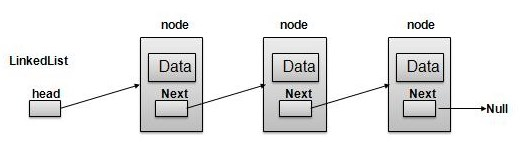
\includegraphics[scale=0.8]{OgP3r.jpg}

También tiene diferentes funcionalidades que fueron implementadas, entre ellas:

\begin{itemize}
	\item add()
	\item remove()
	\item size()
	\item toArray()
\end{itemize}
%----------------------------------------------------------------------------------------


%------------------------------------------------

\subsection*{Media}



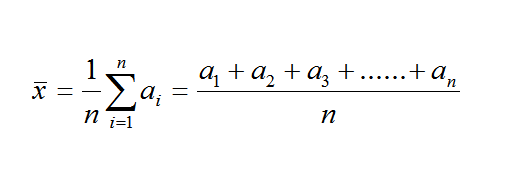
\includegraphics[scale=0.8]{formula-media.png}


Cuando buscamos la media de un conjunto de datos, ubicamos la posición del centro de estos a través del promedio de estos.

La clase Calculator en el repositorio posee un método ( calculateMean() ) 

\begin{verbatim}
public static Double calculateMean(Double[] array){
        Double sum = 0d;
        int n = array.length;
        for(Double x: array) {
            sum += x;
        }
        return sum/n;
    }
\end{verbatim}

Donde, se usó un ciclo For para recorrer los datos y se lleva una variable (sum) para realizar la suma de los datos; se concluye después de recorrer los datos, la media, calculando con el valor n de la cantidad de datos que existen y la suma de todos los datos.

%----------------------------------------------------------------------------------------
\subsection*{Desviación Estándar}

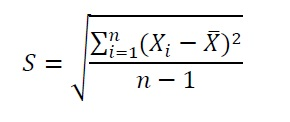
\includegraphics[scale=0.8]{2583684_orig.jpg}

La desviación estándar cuantifica la variación de la población, aunque parecería más robusta con respecto a el promedio si se calculara a papel y lápiz, podría ser un procedimiento complejo.

Se implemento un método en la clase Calculator para calcular la desviación estándar ( calculateDeviation() ) 

\begin{verbatim}
public static Double calculateDeviation(Double[] array, double mean){
        Double sumax = 0d;
        int n = array.length;
        for(Double x: array){
            sumax+=Math.pow(x-mean, 2);
        }
        return Math.sqrt((sumax/(n-1)));
    }
\end{verbatim}

Esta vez, usamos el ciclo For para determinar la parte interna de la raíz, donde se llevó una variable (sumax) donde se hacia el cálculo entre el promedio y cada dato del conjunto de datos. El método finaliza retornando la raíz cuadrada de la parte interna de la raíz, usando la librería Math de Java.


%------------------------------------------------

\subsection*{Error Absoluto} 

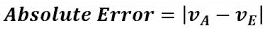
\includegraphics[scale=0.8]{Capture.JPG}


Para poder comprobar nuestros cálculos, necesitamos usar el error absoluto y tener un margen de tolerancia, ya que con este podemos decir si el dato resultante es confiable o no.

\begin{verbatim}
private static Double TOLERANCE=0.1d;

@Test
public void shouldCalculateMean(){
    String file = "src\\test\\resources\\data\\data1.txt";
    LinkedList list = new LinkedList();
    Calculator.readFile(file, list);
    Double errorAbsoluto=Math.abs(Calculator.calculateMean(list.toArray())-
                                    550.6);
    assertTrue(errorAbsoluto < TOLERANCE);
}
\end{verbatim}

Para este caso de prueba, previamente se ha declarado la variable ( TOLERANCE ) para después compararla con el error absoluto.
Usamos el archivo data1.txt que posee un conjunto de datos a operar, guardamos estos datos en la LinkedList para luego determinar la media de estos datos.
En la variable ( errorAbsoluto ) la librería Math se encarga de darnos el valor absoluto entre el valor que se calculó a través de la aplicación y el número que se supone previamente debería dar , después de hacer el cálculo.
Con una tolerancia de 0.1, usamos la variable ( errorAbsoluto )para determinar si el error es menor a la tolerancia que tenemos.
%----------------------------------------------------------------------------------------


\subsection*{Conclusión}

Aunque desde el principio, el taller parecía bastante sencillo, fue un verdadero reto cuando se tuvo que enfatizar en que lo que importaba era la arquitectura del repositorio; y sin dejar de lado la ejecución del programa, se diera a conocer de manera clara y concisa la estructura del repositorio y sus respectivas componentes.

%----------------------------------------------------------------------------------------

\end{document}
